\chapter{Background}\
\label{chap:background}

This section tackles the fundamental principles and groundwork of the theory encompassing concepts, terminology, and methodologies related to search engines as applied within this thesis.

\section{The nature of the web}
The web we know today, Web 2.0, is known as "the participative social web" and is massive, and its rate of change is enormous due to its highly dynamic content. Due to this big sample space, finding the relevant pages or documents from the web isn't easy. To overcome this issue, there are two main approaches to sampling: 
Vertical sampling: Focus only on the pages that are restricted by the domain name. This can be done in different levels. For example, one can restrict the crawling process based on the country, such as .de, .ly, uk. When vertical sampling is done at the second level, it limits the crawling to domains (e.g. stanford.edu) [3].
Horizontal sampling: In this approach, it is important to know the most visited pages and domains to keep crawling from them, giving them more priority than others. This can be done by collecting data logs from the ISP or utilising a web crawler to estimate the page's popularity [3]. 


\section{History}
\numberwithin{equation}{chapter}

The World Wide Web is an unlimited space to share provide and share information. Those information can have different format and cover different doamins. The use case of the web is only limtied by the developers imagination. This is benifital as the Web keept evolving rapidaly form Web 1.0 to Web 2.0 to Web 3.0. Web 1.0 used static pages to serve information, those information were moslty news, blogs and personal langing pages. Some refre to the Web 1.0 as "the read-only web". Although Web 1.0 was massive however most content were created was by deverlopers or at least users who knew basics of the HTML and CSS, moreover by that time content were only static they did not depen on fancy JavaScript libraries and frameworks like Angular and React, this made it limited to some use cases only. Fast forward, pages become more dynamic after using sessions, databases and clint rendering schemas. Those changes made the Web focused not only reading and gathering information by gave the power to more audiounce who did not know any programming or coding to participate and interact with the Web via browsers. Social media, e-commerce and trading stocks platforms was one of the reasons made the internet buble inflate, Use cases where unlimited as useres could create and deploy their own websites by using simple tools as Content Manament System CMS. This made Web 2.0 known as "the participative social web".

To optimize the allocation of crawler resources, estimating the page's freshness must be considered. This prevents outdated pages from remaining unrefreshed for prolonged periods or where lesser-significant pages are needlessly recrawled despite unchanged content.


It can be understood intuitively that the likelihood of a copy of page p being up-to-date at time t, denoted as up(t), declines over time when the page is not revisited.

\begin{equation}
u_p(t) \propto e^{-\lambda_pt}
\label{eq:depth}
\end{equation}

The parameter λp signifies the rate of modifications occurring on page p, and its estimation can be deduced from past observations, mainly when the web server indicates the page's last modification date during visits. Cho and Garcia-Molina derived this estimation technique for λp [8].

\begin{equation}
\lambda_p \approx \frac{(X_p-1) - \frac{X_p}{N_p\log(1-X_p/N_p)}}{S_pT}
\label{eq:depth}
\end{equation}

\begin{itemize}
  \item Np number of visits to p.  
  \item Sp time since the first visit to p.
\item Xp number of times the server has informed that the page has changed.
\item Tp total time with no modification, according to the server, summed over all the visits.
\end{itemize}

Note that some pages do not include the last-modified time stamp, and in this case, one can estimate this manually by comparing the
downloaded copies at two different times and using the following equation. Where Xp now will be the number of times a modification is detected.

\begin{equation}
\lambda_p \approx \frac{-N_p\log(1-X_p/N_p)}{S_p}
\label{eq:depth}
\end{equation}

\section{Web Search Engine}
Web Search Engine is software that collects information from the web and indexes them efficiently to optimize the searching process by the user. Users enter their queries to ask for information. The engine performs queries, looks up the pre-built organized index, and returns relevant results. The returned result is presented by Search Engine Results Pages as known as SERPs. The result is then ranked based on predefined criteria. 

Web search engines use web crawlers or spiders to collect and harvest the internet jumping from one page to another. Each page can contain several links. The crawler's task is to find the links, visit them, and harvest them. Followed by crawlers, indexing is the next process where information is organized and optimized for search. 

\begin{figure}[h]	
     \centering
         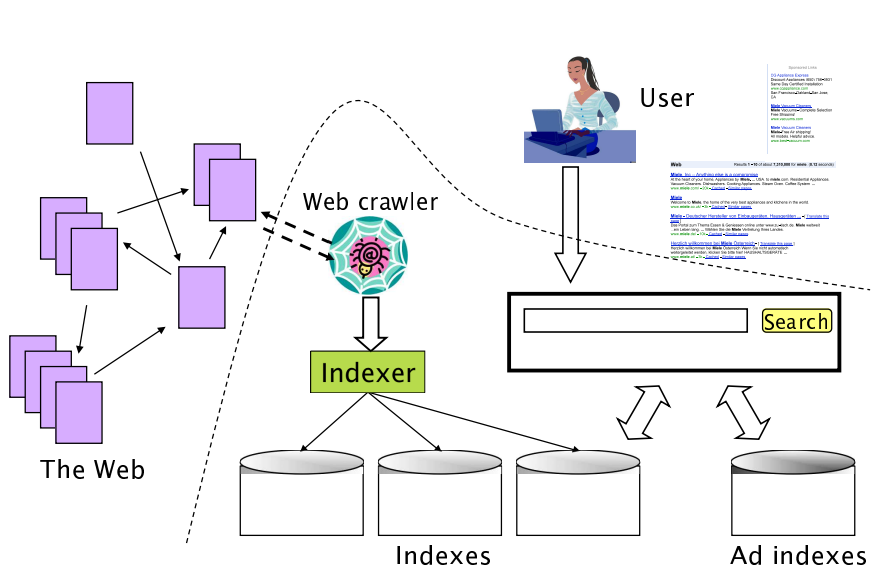
\includegraphics[width=10cm]{images/engine_components.png}
\end{figure}

\subsection{Requierments and Features}
Search engines, regardless of their imp[lmentation and design there, are some features and requirements that make a good one; following is a list of the most fundamentals features:  

\begin{itemize}
  \item Web Crawling and Indexing: Each search engine needs two main big components, Crawler and Indexer. The Crawler is the component responsible for collecting pages and downloading them from the web. An indexer is used to create an index to facilitate efficient searching.
  \item Ranking and Relevancy: The algorithm determines the order in which search results are presented to users based on relevance.
  \item User Interface: The user interface where users enter their search queries and view results.
  \item Scalability and Performance: Distributed Architecture: A distributed system helps handle the vast amount of data and traffic. This needs a Load balancer to distribute the cralwing tasks betrween the nodes and threads. 
  \item Data Storage and Management: A robust database system is necessary for storing indexed data and metadata.
\end{itemize}

\section{Cralwer}
Web crawler or spidedr is a software which gather pages information from the web, to prived the neccasary datat to the indexer to build a searhc engine. The essintial role of crawlers is to effecitnalt and reliably collect as much infromation from the web. 

\section{Cralwer Specifications}
Crawlers can have a wide vireity of features and specifications, however some are necessary to include and others are vital to have a reliable useable one. 

\begin{itemize}
  \item Robustness: Web crawler can be fragile and easy to break, this is due to the nature of the dynamic contnets on the web and the internet connection. Web crawlers must identify those edge cases and obsticals and tackle them.  
  \item Politeness: The implmentation of the crawler can be unintentially mellisous and dangerous if not designed correclty. A Deniel of service DoS and a Distributed Denial of service DDoS attacks can occure due to a bad crawler implmentation. Hence crawlers must respect websites policies and avoid breaking up web services and load the servers.

\item Distributed: To make the crawler efficint and 

The crawler should have the ability to execute in a distributed
fashion across multiple machines.
\end{itemize}


\\



Scalable: The crawler architecture should permit scaling up the crawl rate
by adding extra machines and bandwidth.
Performance and efficiency: The crawl system should make efficient use of
various system resources including processor, storage and network bandwidth.
Quality: Given that a significant fraction of all web pages are of poor utility for serving user query needs, the crawler should be biased towards
fetching “useful” pages first.
Freshness: In many applications, the crawler should operate in continuous
mode: it should obtain fresh copies of previously fetched pages. A search
engine crawler, for instance, can thus ensure that the search engine’s index
contains a fairly current representation of each indexed web page. For
such continuous crawling, a crawler should be able to crawl a page with
a frequency that approximates the rate of change of that page.
Extensible: Crawlers should be designed to be extensible in many ways –
to cope with new data formats, new fetch protocols, and so on. This demands that the crawler architecture be modular.

\section{Indexing}
2.4 Web crawling issues page 27 book Effective Web Crawling by Carlos Castillo
